\documentclass[11pt,a4paper]{article}

\usepackage[utf8]{inputenc}
\usepackage[T1]{fontenc}
\usepackage{lmodern}
\usepackage[margin=1in]{geometry}
\usepackage{graphicx}
\usepackage{hyperref}
\usepackage{xcolor}
\usepackage{titlesec}
\usepackage{float}
\usepackage{parskip}
\usepackage{fancyhdr}
\usepackage{enumitem}

% Define colors
\definecolor{primary}{RGB}{30, 136, 229}
\definecolor{secondary}{RGB}{21, 101, 192}
\definecolor{highlight}{RGB}{200, 230, 255}

% Setup links
\hypersetup{colorlinks=true,linkcolor=primary,urlcolor=primary}

\pagestyle{fancy}
\fancyhf{}
\rhead{Panduan Lengkap Pengguna \& Alur Kerja}
\lhead{Aplikasi Putra Remaja}
\cfoot{\thepage}

\titleformat{\section}{\Large\bfseries\color{primary}}{}{0em}{}[\titlerule]
\titleformat{\subsection}{\large\bfseries\color{secondary}}{}{0em}{}
\titleformat{\subsubsection}{\normalsize\bfseries}{}{0em}{}

\begin{document}

\begin{titlepage}
    \centering
    \vspace*{2cm}
    {\Huge \textbf{\textcolor{primary}{Panduan Lengkap Alur Kerja Aplikasi}}}\\[1.5cm]
    {\LARGE \textbf{Penjelasan Langkah-Demi-Langkah Per-Peran Sesuai Sistem}}}\\[1cm]
    \vfill
    {\Large \textbf{Sistem Manajemen Tiket \& Operasional Bus}}\\[0.5cm]
    {\large Disusun Secara Otomatis -- \today}\\[2cm]
\end{titlepage}

\clearpage
\tableofcontents
\clearpage

\section{Pendahuluan: Hak Akses Resmi di Dalam Sistem}
Sistem aplikasi membedakan wewenang dan jenis pekerjaan manusia ke dalam 8 (delapan) peran (\textit{Role}) yang sah tercatat di dalam Database Utama. Masing-masing peran akan membawa tanggung jawab spesifik pada setiap tahapan kerja yang berbeda:
\begin{enumerate}
    \item \textbf{Superadmin}: Pemegang kunci utama dari sistem, sanggup membuat rute baru dan melihat data paling mendasar.
    \item \textbf{Management}: Pimpinan perusahaan. Terfokus murni pada membaca hasil penjualan atau laba dari layar laporan harian/bulanan.
    \item \textbf{ADMIN}: Bagian operasional pabrik jadwal. Tugasnya menyusun rentang keberangkatan bus dan memberangkatkan setiap armada kepada penumpang.
    \item \textbf{CS} (Customer Service): Pekerja garda depan yang melayani penumpang, mencocokkan bangku kosong, dan mengurusi pesanan masuk.
    \item \textbf{Reservasi}: Bersifat mirip dengan \textbf{CS}, mereka membantu mengunci (booking) tiket dan memasukkan biodata.
    \item \textbf{Agent}: Pemesan lepas atau cabang agen mitra resmi yang menjual tiket keberangkatan di layar mereka.
    \item \textbf{CASHIER}: Kasir garasi operasional. Memberikan bekal tunai pada supir sebelum jalan dan menyalin bon tagihan tol tatkala supir pulang kembali.
    \item \textbf{FINANCE}: Sang auditor ujung. Memastikan bon \textbf{CASHIER} memang tepat lalu menyetujui pemotongan saldo nyata di buku perusahaan.
\end{enumerate}

\clearpage
\section{1. Tahap Persiapan \& Pembuatan Jadwal (Preparation)}
Sebelum ada selembar tiket pun yang bisa dijual ke pelanggan di loket manapun, bagian operasional Pusat perlu "memproduksi barang jadwal"-nya terlebih dahulu.

\subsection{1.1 Penjelasan Langkah Demi Langkah}
\textbf{Langkah 1: Peran `Superadmin` -- Mendata Rute Dasar}
Sebelum jadwal dibikin, \textbf{Superadmin} masuk ke menu \textbf{"Master Armada \& Rute"}. Superadmin menentukan data relasi rute (contoh: Jogja - Jakarta) dan berapa kursi bus yang dimainkan (Misal tipe 30 Bangku). Ini akan tersimpan mantap sebagai Master Data.

\textbf{Langkah 2: Peran `ADMIN` -- Memilih Rute dan Penjadwalan Panjang}
Kini giliran \textbf{ADMIN} (Operasional) yang memasuki menu bernama \textbf{"Dashboard Penjadwalan"}.
\begin{itemize}[leftmargin=1.5cm]
    \item \textbf{ADMIN} meng-klik tombol \textbf{"Tambah"}.
    \item Di layar muncul pilihan. \textbf{ADMIN} mengetik \textit{Nama Jadwal}, memastikan pilihan \textit{Rute}, dan menyetel \textit{Rentang Tanggal} (contoh: 1 s.d. 30 September).
    \item \textbf{ADMIN} lantas meng-klik tombol \textbf{"Generate Jadwal"}. Begitu diklik, sistem aplikasi akan langsung otomatis memecah kalender mencetak slot jadwal persis tiap harinya tanpa perlu diketik hari per hari.
\end{itemize}

\textbf{Langkah 3: Peran `ADMIN` -- Menugaskan Sang Supir}
Sekarang, sistem sudah memiliki slot bus harian. \textbf{ADMIN} masuk ke lembar \textbf{"Jadwal Bus Harian"}.
\begin{itemize}[leftmargin=1.5cm]
    \item \textbf{ADMIN} membuka bus untuk keberangkatan khusus besok pagi.
    \item Di form tersebut, \textbf{ADMIN} memutuskan dan mengisi \textbf{"Nama Supir"} pada kolom Supir.
    \item \textbf{ADMIN} menutupnya dengan klik \textbf{"Simpan"}. Setelah nama supir tersimpan, status armada ini segera dibuka menjadi "Siap Dipesan" dan secara instan pula akan muncul di seluruh layar para \textbf{Agent}.
\end{itemize}

\subsection{1.2 Bagan Urutan Kerja (Tahap Persiapan)}
\begin{figure}[H]
    \centering
    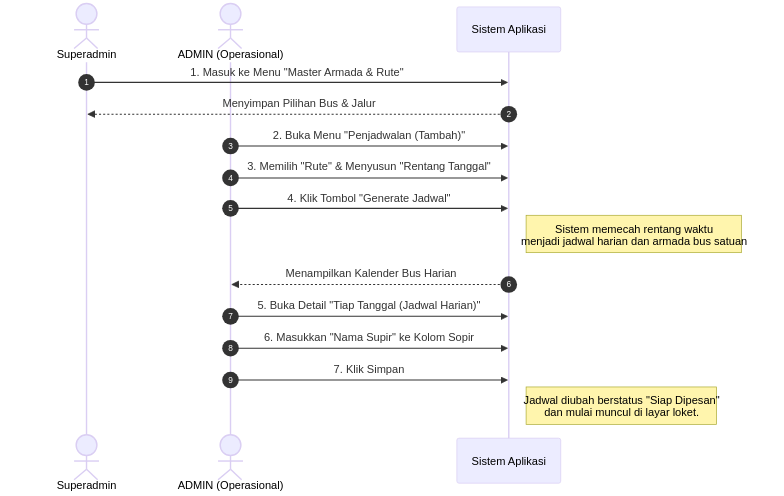
\includegraphics[width=\textwidth,height=0.55\textheight,keepaspectratio]{images/prep_sequence.png}
    \caption{Kerjasama Transisi Superadmin Menaruh Rute \& ADMIN Meluncurkan Jadwal}
\end{figure}

\clearpage
\section{2. Tahap Transaksi \& Penjualan Lintas Loket (Booking)}
Armada jadwal telah tercipta, loket pun dibuka. Penumpang tiba dan dilayani di layar cabang masing-masing.

\subsection{2.1 Penjelasan Langkah Demi Langkah}
\textbf{Langkah 1: Peran `CS` / `Reservasi` / `Agent` -- Mencari Rangkaian Bus Bersedia}
Pelanggan datang. Penjaga loket dengan akun ber-Role \textbf{CS} atau \textbf{Agent} segera bertugas.
\begin{itemize}[leftmargin=1.5cm]
    \item \textbf{CS} berpindah ke Menu \textbf{"Reservasi Tiket"}.
    \item \textbf{CS} mengisi keterangan \textbf{"Tanggal Keberangkatan"} dan menyetel tempat pemberangkatan (Misal: Agen Jombor).
    \item \textbf{CS} menekan tombol \textbf{"Cari"}. Dalam waktu singkat, aplikasi menyajikan cetak biru denah kursi bus kosong (hasil keringat proses \textbf{ADMIN} awal tadi).
\end{itemize}

\textbf{Langkah 2: Peran `CS` / `Reservasi` / `Agent` -- Mengambil \& Mengunci Kursi (Locking)}
\begin{itemize}[leftmargin=1.5cm]
    \item \textbf{CS} mengarahkan tangannya ke \textit{mouse} lalu menunjuk bangku nomor \textbf{"4A"}.
    \item \textbf{PENTING:} Saat \textbf{CS} mengekliknya, sistem menyadari perbuatan ini dan segera menguncinya! Di layar \textbf{Agent} lain di kota berbeda, bangku nomor 4A auto berubah warna abu-abu. Resiko tabrakan tiket (\textit{Double Book}) pun berhasil musnah.
\end{itemize}

\textbf{Langkah 3: Peran `CS` / `Reservasi` -- Mencatat Biodata Identitas}
Setelah aman terkunci, \textbf{CS} melengkapi sisanya:
\begin{itemize}[leftmargin=1.5cm]
    \item \textbf{CS} melengkapi isian teks \textbf{"Nama Penumpang"} dan \textbf{"Nomor Handphone"}.
    \item Lalu, \textbf{CS} membenturkan klik pada tombol \textbf{"Hitung Total Harga"} dan aplikasi membaca sendiri tarif tambahan manakala ini adalah musim liburan.
\end{itemize}

\textbf{Langkah 4: Bayar Lunas di Tempat}
\begin{itemize}[leftmargin=1.5cm]
    \item \textbf{CS} mengambil uang pelanggan dan memilih Tipe Pembayaran \textbf{"Tunai / Lunas"}.
    \item Terakhir tekan kuat di bagian klik \textbf{"Pesan \& Lunas"}.
    \item Layar layar \textbf{CS} menukar keterangan status milik pelanggan dengan stempel "BAYAR (PAID)". Pemesanan final terpenuhi penuh.
\end{itemize}

\subsection{2.2 Bagan Urutan Kerja (Tahap Transaksi Reservasi)}
\begin{figure}[H]
    \centering
    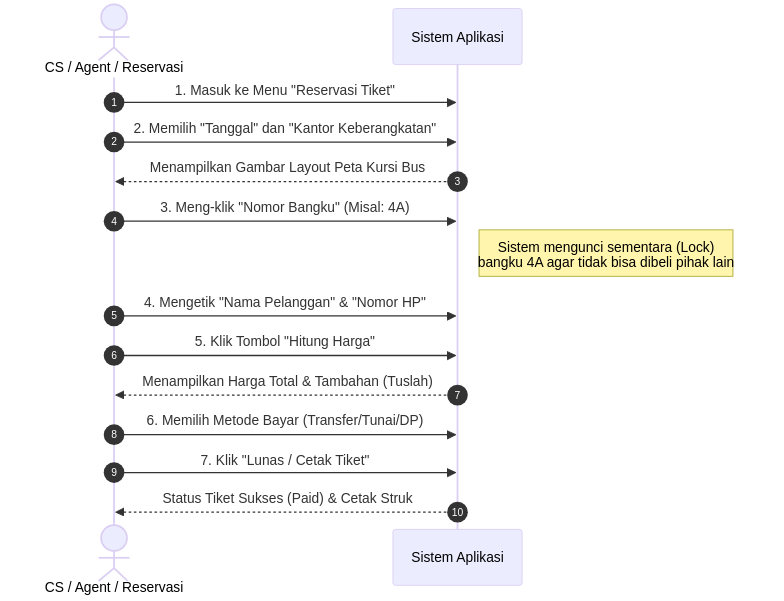
\includegraphics[width=\textwidth,height=0.55\textheight,keepaspectratio]{images/booking_sequence.png}
    \caption{Alur Penjualan Agen: Mengunci Bangku, Mengambil Biodata dan Menerima Pelunasan}
\end{figure}

\clearpage
\section{3. Tahap Pemantauan Hasil (Tahap Laporan Cepat)}
Sepanjang siang saat para \textbf{CS} / \textbf{Agent} sibuk mengubah penjualan menjadi saldo "PAID", secara magis hasil tersebut diam-diam terbang langsung ke ranah analisis tanpa campur tangan mereka.

\subsection{3.1 Penjelasan Langkah Demi Langkah}
\textbf{Langkah 1: Rekam Otomatis Oleh Skema Mesin}
Tepat di hitungan kelip sedetik sejak tiket berganti stempel menjadi dibayar, layar sistem mencatat pertambahannya sendiri (\textit{"Pendapatan Agen A naik, pendapatan Traveloka bertambah"}). Tak ada satupun peran manusia yang bekerja menginput data ini ke laci laporan lagi.

\textbf{Langkah 2: Peran `Management` / `Superadmin` -- Membaca Visual Laporan Laba}
Sesosok pemegang akun \textbf{Management} memantau perkembangan perusahaan di sore hari via ruangan mereka.
\begin{itemize}[leftmargin=1.5cm]
    \item \textbf{Management} login secara rahasia dan menavigasi klik ke layar grafik \textbf{"Laporan Keseluruhan"}.
    \item Pejabat \textbf{Management} menyetel \textit{dropdown} rentang hari dan menunjuk area spesialis waktu: \textbf{"Bulan Lalu"}.
    \item \textbf{Management} menembakkan klik padanya: \textbf{"Terapkan Carian"}.
\end{itemize}

\textbf{Langkah 3: Visual Layar Kilat}
Sesaat kemudian mesin menampilkan grafik analitik bundar Kue (Pie) untuk melihat pertempuran saluran pemasukan daring melawan pemesanan manual, semuanya mulus tampil tanpa layar lambat karena rekap uangnya dicatat nyicil semenjak langkah transaksi yang kecil-kecil tadinya.

\subsection{3.2 Bagan Urutan Kerja (Tahap Laporan Ringkasan)}
\begin{figure}[H]
    \centering
    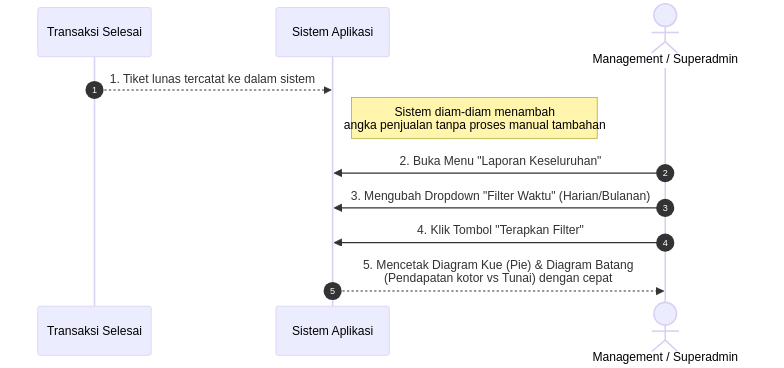
\includegraphics[width=\textwidth,height=0.55\textheight,keepaspectratio]{images/report_sequence.png}
    \caption{Role Management Melancarkan Aksi Membaca Grafik Pencari Rekap Cepat Database}
\end{figure}

\clearpage
\section{4. Tahap Pengecekan Bon Eksternal Lapangan (Finance)}
Estafet paling akhir dalam putaran ini ada di lorong garasi bus dan lorong bank. Tiketnya memang sudah habis terjual, dan supir pun menjalankan armada secara fisik. Uang bensin harus dikeluarkan dengan akurat.

\subsection{4.1 Penjelasan Langkah Demi Langkah}
\textbf{Langkah 1: Peran `CASHIER` -- Memberi Awalan Uang Saku}
Beberapa jam sebelum kunci kontak armada ditarik:
\begin{itemize}[leftmargin=1.5cm]
    \item Pekerja \textbf{CASHIER} garasi memasuki halaman form \textbf{"Uang Saku"}.
    \item \textbf{CASHIER} mengisikan nama bus dan merogoh uang bernilai dasar Rp 1.000.000 via log komputer lalu membuahkan tombol \textbf{"Simpan"}. Pecahan fisik dari nilai ini diangsur ke tangan sang supir tersebut. Supir lantas pergi bekerja ke luar kota.
\end{itemize}

\textbf{Langkah 2: Proses Kedatangan Bawaan Surat Fisik (\textit{Bon})}
Di ujung lusa, supir kembali merapat di terminal yang sama. Pak supir turun bermodalkan struk minyak, bon cuci mobil, serta selembar struk kuning portal Tol.

\textbf{Langkah 3: Peran `CASHIER` -- Menu Input Pemasukan Bukti Draf Riil}
\begin{itemize}[leftmargin=1.5cm]
    \item \textbf{CASHIER} sigap menuju menu form selanjutnya yang bernama \textbf{"Realisasi Keberangkatan"}.
    \item Di sana \textbf{CASHIER} menatap kertas asli dan menyalin ke layar: \textbf{Ongkos BBM:} Rp 600.000, serta angka \textbf{Ongkos Tol} di sebelahnya sesuai kenyataan aslinya.
    \item Seturutnya \textbf{CASHIER} memejat mantap penegasan penyerahan via klik \textbf{"Simpan Bukti (Draft)"}. Aplikasi menyurati rekam buktinya tetapi ingat, uang keseluruhan di laporan korporasi perihal \textbf{Management} tadi belum terpotong sepeserpun! Ia digantung terlebih dahulu demi keamanan.
\end{itemize}

\textbf{Langkah 4: Peran `FINANCE` -- Tahapan Verifikasi Final Dan Pemotongan Mutlak}
Tugas tangan kasar putus di sini. Babak akhir dilanjutkan pemegang lisensi tertinggi keuangan.
\begin{itemize}[leftmargin=1.5cm]
    \item Individu \textbf{FINANCE} korporate menyelami daftar draf pengeluaran kasir ini melelalui kamar persetujuan khusus miliknya bernama \textbf{"Lembar Pengecekan Buku / Ledger"}.
    \item \textbf{FINANCE} menanding silang log dari draf sang Cashier sebelumnya.
    \item Jika segala nilai serasa jernih dan benar, petugas \textbf{FINANCE} menjatuhkan sanksi akhirnya -- menggores tombol putusan \textbf{"Tindakan Posting Final"}!
    \item Ketuk konfirmasi ini menjadi lonceng terakhir di mana brankas perusahaan setuju untuk dipotong dengan sah guna operasional, menuntaskan dan menge-lem lembaran catatan perjalanan gerbong bus ini selamanya dalam rekor perusahaan.
\end{itemize}

\subsection{4.2 Bagan Urutan Kerja (Tahap Validasi Ledger Keuangan)}
\begin{figure}[H]
    \centering
    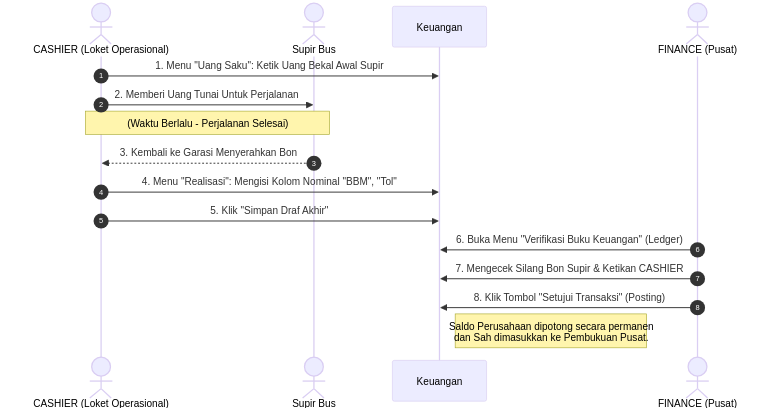
\includegraphics[width=\textwidth,height=0.55\textheight,keepaspectratio]{images/finance_sequence.png}
    \caption{Tongkat Tanggung Jawab Dari Uang Saku CASHIER Diambil Alih Tuntas Oleh Posting FINANCE}
\end{figure}

\end{document}
